\documentclass[
    % -- opções da classe memoir --
    12pt,               % tamanho da fonte
    openright,          % capítulos começam em pág ímpar (insere página vazia caso preciso)
    oneside,            % para impressão em verso e anverso. Oposto a oneside
    a4paper,            % tamanho do papel.
    % -- opções da classe abntex2 --
    chapter=TITLE,      % títulos de capítulos convertidos em letras maiúsculas
    section=TITLE,      % títulos de seções convertidos em letras maiúsculas
    % -- opções do pacote babel --
    english,
    brazil              % o último idioma é o principal do documento
]{abntex2}

\usepackage[T1]{fontenc}    % Selecao de codigos de fonte.
\usepackage[utf8]{inputenc} % Codificacao do documento (conversão automática dos acentos)
\usepackage{lastpage}       % Usado pela Ficha catalográfica
\usepackage{indentfirst}    % Indenta o primeiro parágrafo de cada seção.
\usepackage{color}          % Controle das cores
\usepackage{microtype}      % para melhorias de justificação
\usepackage{listings}       % para inserir código fonte
\usepackage{graphicx}       % para inserir imagens
\usepackage{enumitem}

% Pacotes de citações
\usepackage[brazilian,hyperpageref]{backref} % Paginas com as citações na bibl
\usepackage[alf]{abntex2cite} % Citações padrão ABNT
\usepackage{titlesec}

\usepackage{tikz}
\usetikzlibrary{shapes,arrows,shadows}

\pgfdeclarelayer{background}
\pgfdeclarelayer{foreground}
\pgfsetlayers{background,main,foreground}

% ---
% CONFIGURAÇÕES DE PACOTES
% ---

% altera o espacamento depois do número de cada secao, subsecao, etc
\titleformat{\section}
  {\normalfont\normalsize}{}{0pt}{\thesection\space}
\titleformat{\subsection}
  {\normalfont\normalsize\bfseries}{}{0pt}{\thesubsection\space}
\titleformat{\subsubsection}
  {\normalfont\normalsize}{}{0pt}{\thesubsubsection\space}
\titleformat{\paragraph}
  {\normalfont\normalsize\itshape}{}{0pt}{\theparagraph\space}

% ---
% Configurações do pacote backref
% Usado sem a opção hyperpageref de backref
\renewcommand{\backrefpagesname}{Citado na(s) página(s):~}
% Texto padrão antes do número das páginas
\renewcommand{\backref}{}
% Define os textos da citação
\renewcommand*{\backrefalt}[4]{
    \ifcase #1 %
        Nenhuma citação no texto.%
    \or
        Citado na página #2.%
    \else
        Citado #1 vezes nas páginas #2.%
    \fi}%
% ---

% ---
\titulo{\uppercase{Uma proposta de interface do cliente de torrent Transmission
                   baseado no GTK HIG 3.14}}
\autor{\uppercase{Derek Willian Stavis}}
\orientador{Prof. Luciana Schmitz, Esp. (SENAI/SC)}
\orientadortcc{Prof. \imprimirorientador, Dr. (SENAI/SC)}
\coordenador{Prof. Luciana Schmitz, Esp. (SENAI/SC)}
\coordenadortcc{Profa. Aline Cristina Antonelli de Oliveira, Esp. (SENAI/SC)}
\examinador{Prof. João Carlos Testi Ferreira, Esp. (SENAI/SC)}
\preambulo{Trabalho de Conclusão de Curso apresentado à Banca Examinadora do
           Curso Superior de Tecnologia em Análise e Desenvolvimento de Sistemas
           da Faculdade de Tecnologia do SENAI Florianópolis como requisito
           parcial para obtenção do Grau de Tecnólogo em Análise e
           Desenvolvimento de Sistemas.}
\proforientador{Professor Orientador: \imprimirorientador.}
\datadefesa{\uppercase{18 de Dezembro de 2015}}
\local{Florianópolis/SC}
\data{2015}

\instituicao{%
  SERVIÇO NACIONAL DE APRENDIZAGEM INDUSTRIAL
  \par
  FACULDADE DE TECNOLOGIA SENAI/SC FLORIANÓPOLIS
  \par
  CURSO SUPERIOR DE TECNOLOGIA EM ANÁLISE E DESENVOLVIMENTO DE SISTEMAS}
\tipotrabalho{Trabalho de Conclusão de Curso}

% alterando o aspecto da cor azul
\definecolor{blue}{RGB}{41,5,195}

% informações do PDF
\makeatletter
\hypersetup{
        %pagebackref=true,
        pdftitle={\@title},
        pdfauthor={\@author},
        pdfsubject={\imprimirpreambulo},
        pdfcreator={LaTeX with abnTeX2},
        pdfkeywords={torrent client}{transmission}{gnome}{gtk}{redesign}{interface},
        colorlinks=true,    % false: boxed links; true: colored links
        linkcolor=black,    % color of internal links
        citecolor=black,    % color of links to bibliography
        filecolor=magenta,  % color of file links
        urlcolor=black,
        bookmarksdepth=4
}
\makeatother
% ---

% ---
% Espaçamentos entre linhas e parágrafos
% ---

% O tamanho do parágrafo é dado por:
\setlength{\parindent}{1.3cm}

% Controle do espaçamento entre um parágrafo e outro:
\setlength{\parskip}{0.2cm}  % tente também \onelineskip

%\titlespacing\section{0pt}{12pt plus 4pt minus 2pt}{-6pt plus 2pt minus 2pt}

% ---
% compila o indice
% ---
\makeindex
% ---

% ----
% Início do documento
% ----
\begin{document}

% Retira espaço extra obsoleto entre as frases.
\frenchspacing

% ----------------------------------------------------------
% ELEMENTOS PRÉ-TEXTUAIS
% ----------------------------------------------------------

\imprimircapa
\imprimirfolhaderosto*

\begin{folhadeaprovacao}

  \begin{center}
    {\ABNTEXchapterfont\bfseries\normalsize\imprimirautor}

    \vspace*{\fill}\vspace*{\fill}
    \begin{center}
      \ABNTEXchapterfont\bfseries\normalsize\imprimirtitulo
    \end{center}
    \vspace*{\fill}
        \imprimirpreambulo
    \vspace*{\fill}

   APROVADA PELA {\bfseries{COMISSÃO EXAMINADORA}}
   \par
   EM FLORIANÓPOLIS, \bfseries{\imprimirdatadefesa}
   \end{center}

   \assinatura{\imprimircoordenador \\ Coordenador do Curso}
   \assinatura{\imprimircoordenadortcc \\ Coordenador de TCC}
   \assinatura{\imprimirorientadortcc \\ Orientador}
   \assinatura{\imprimirexaminador \\ Examinador}
   \begin{center}
    \vspace*{1cm}
  \end{center}
\end{folhadeaprovacao}

% ====================================================================
% Epigrafe 
% ====================================================================
\begin{epigrafe}
    \vspace*{\fill}
	\begin{flushright}
		\textit{``Que os vossos esforços desafiem as impossibilidades, lembrai-vos de que as \\
		grandes coisas do homem foram conquistadas do que parecia impossível''} \\
		(CHARLES CHAPLIN)
	\end{flushright}
\end{epigrafe}


\noindent STAVIS, Derek Willian. \textbf{\imprimirtitulo} Florianópolis, 2015.
\pageref{nropaginas}f. Trabalho de Conclusão de Curso Superior de Tecnologia em
Análise e Desenvolvimento de Sistemas. Faculdade de Tecnologia do SENAI,
Florianópolis, 2015.

\vspace{1cm}
\setlength{\absparsep}{18pt} % ajusta o espaçamento dos parágrafos do resumo
\begin{resumo}

  Os avanços trazidos nos últimos quatro anos no ambiente gráfico GNOME foram de
  suma importância para atingir uma experiência diferenciada e consistente de
  uso. Conceitos já difundidos no design de interfaces de usuário foram
  revisitados, paradigmas foram quebrados, mudando a forma com que os usuários
  vêem e interagem com o sistema operacional. Entretanto, nem todos os softwares
  disponíveis para a plataforma acompanharam a velocidade de desenvolvimento da
  plataforma GNOME, e muitos ainda necessitam de atenção. Com o lançamento do
  HIG (Guia de Interface com o Usuário) no GNOME versão 3.12 toda filosofia e
  padrões de design da plataforma foram sintetizados em linguagem simples e
  objetiva, tornando-se o material referência para o desenvolvimento e
  manutenção de seu ecosistema de softwares. Esta pesquisa aborda o processo de
  adaptação do cliente de torrent Transmission de acordo com o guia de
  interfaces do GNOME versão 3.14.

  \vspace{\onelineskip}

  \noindent
  \textbf{Palavras-chave}: Interfaces Gráficas. GTK+. GNOME. Design. Redesign.

\end{resumo}

\noindent STAVIS, Derek Willian. \textbf{\imprimirtitulo} Florianópolis, 2013.
\pageref{nropaginas}f. Trabalho de Conclusão de Curso Superior de Tecnologia em
Análise e Desenvolvimento de Sistemas. Faculdade de Tecnologia do SENAI,
Florianópolis, 2013.

\vspace{1cm}
\begin{resumo}[\textbf{ABSTRACT}]
 \begin{otherlanguage*}{english}
   
  The advances in the last four years in GNOME Desktop Environment was utmost to
  achieve a consistent and distinguished user experience. Widespread concepts
  already used in user interface design were revisited and paradigms were
  broken, thus changing how the user see and interact with a computer. Although,
  not every software available for the GNOME desktop followed with the
  transition period, and most softwares needs attention.
  
  With the release of GNOME Human Interface Guidelines together with version
  3.12 of GNOME as a official documentation for design principles, all
  platform's philosophies and design patterns were translated in a simple and
  objective language, aiming to be the reference for both development and 
  maintenance of GNOME's ecosystem.

  This research addresses the thinking process of redesigning the user interface
  of Transmission, a free and open source client for file sharing, targeting
  GNOME HIG version 3.14.

   \vspace{\onelineskip}
 
   \noindent 
   \textbf{Key-words}: Graphical User Interfaces. GTK+. GNOME. Design. Redesign.
 \end{otherlanguage*}
\end{resumo}



% lista de figuras
\pdfbookmark[0]{\listfigurename}{lof}
\listoffigures*
\clearpage

% inserir lista de tabelas
\pdfbookmark[0]{\listtablename}{lot}
\listoftables*
\clearpage

\begin{siglas}
  \item[GNU] GNU is Not Unix - Projeto de licenciamento e distribuição de pacotes de software, baseados na licença GNU GPL.
  \item[GPL] General Public License - Modelo de licenciamento de software baseado em liberdades.
  \item[GTK+] GIMP Toolkit - Biblioteca de componentes para criação de interfaces gráficas.
  \item[API] Application-Programmer Interface - Protocolos de comunicação de um determinado pacote de software.
  \item[GIMP] GNU Image Manipulation tool - Ferramenta de manipulações de imagem de código aberto, sob licença GNU.
  \item[GNOME] Ambiente gráfico de estação de trabalho disponível para GNU/Linux.
  \item[HIG] Human Interface Guidelines - Guia de referências de design para implementação de interfaces.
\end{siglas}




% inserir o sumario
\pdfbookmark[0]{\contentsname}{toc}
\tableofcontents*
\clearpage

% ----------------------------------------------------------
% ELEMENTOS TEXTUAIS
% ----------------------------------------------------------
\textual

\chapter{INTRODUÇÃO}

O GNOME é um ambiente gráfico similar aos apresentados pelo Microsoft Windows e
Apple OS X. Com uma experiência de usuário única, o GNOME, diferente de seus
similares proprietários, é mantido por uma comunidade de desenvolvedores aberta
e sua licença de código-fonte permite que virtualmente qualquer pessoa no mundo
possa estudar ou modificar seu funcionamento.

O lançamento de um guia oficial de padrões para o desenvolvimento de interfaces
gráficas orientadas ao GNOME foi de suma importância para alinhar
desenvolvedores aos objetivos do ambiente gráfico. O guia procura trazer
harmonia visual conforme sua implementação, seja através dos aplicativos
centrais -- os primeiros a receber tratamento estético -- ou por aplicativos de
terceiros, que devem se adaptar utilizando o guia como referência.

Aplicativos que não se adequam ao guia passam a apresentar-se defasados,
perdendo pontos em usabilidade e estética, aumentando a taxa de rejeição.
Mantenedores de aplicativos baseados no \textit{toolkit} GTK+ devem, portanto,
dedicar atenção para o fator usabilidade, mantendo-se compatível com o progresso
da plataforma GNOME.

Um aplicativo que sofre deste efeito e necessita dedicação é o Transmission, um
cliente de \textit{torrent} popular, que foi desenvolvido na era GTK+ versão 2,
onde os requisitos, recursos e visão da plataforma GNOME eram diferentes
\cite{gnome221hig}.

\section{OBJETIVOS}

\subsection{Objetivo geral}

Propor adaptações na interface gráfica GTK+ do cliente de torrent Transmission
através da análise de casos de uso de aplicativos centrais da plataforma GNOME,
versão 3.16, e de acordo com as recomendações do HIG versão 3.14, trazendo mais
harmonia para seus utilizadores na plataforma GNOME.

\subsection{Objetivos específicos}

\begin{enumerate}[label=(\alph*)]
  \item Comparar dados evolutivos da interface de aplicações centrais do GNOME.
  \item Identificar pontos de redesign na janela principal do Transmission.
  \item Propor adaptações na interface do Transmission.
\end{enumerate}

1\chapter{REVISÃO DA LITERATURA}

O desenvolvimento de mecanismos que automatizam tarefas existe desde a idade das
pedras, onde hominídeos produziam ferramentas para auxílio próprio. A
transversalidade do conhecimento e da experimentação nos levou a descoberta de
novas metodologias e o aperfeiçoamento de técnicas, consequentemente modificando
a forma com que o ser humano interage com o mundo
\cite[p. 1]{sartori2010neurociencia}.

\section{Interfaces gráficas}

O conceito de interface é extremamente amplo, e foi largamente difundido com o
início dos estudos de interação humano-máquina. O avanço da industrialização
permitiu com que máquinas extremamente complexas substituíssem seres humanos nas
tarefas mais difíceis, deixando estes, seus operadores, apenas com a
responsabilidade de pilotá-las de forma simples e segura.

O advento de tecnologias multimídias interativas como computadores, celulares e
tablets elevou o patamar da criação de interfaces e gestão de tarefas ao estado
da arte, agregando conhecimentos transversais de artistas visuais a músicos.

\citeonline[p. 1]{ferreira2005semiotics} afirmam que a criação de “interfaces
com o usuário ainda está mais para arte do que para ciência.", e justificam,
explicando que "A maior parte do design ou redesign é baseado em estudos
empíricos ou protótipos, e ainda há muito pouca compreensão teórica ou de
engenharia de como conduzir o processo de design e produzir bons designs pela
primeira vez”.

Interfaces gráficas modernas foram alcançadas através da associação entre
hardware e software, podendo utilizar de um ou mais dispositivos de entrada e
saída, com o intuito de promover usabilidade e fácil adaptação.

Dispositivos de entrada transformam coordenadas do mundo real para o mundo
virtual, registrando condições externas que podem ser modificadas através da
interação com um ou mais atores. Dispositivos de entrada comuns são mouse, tela
de toque, teclado, etc.

Dispositivos de saída projetam informações geradas por um sistema computacional
e seu caráter é geralmente baseado nos sentidos: Visão, audição, tato. O
dispositivo de saída mais comum é o monitor, que tem por finalidade projetar
imagens compatíveis com a capacidade humana de visão.

\section{Gerenciadores de Janelas}

Gerenciadores de janelas tem como principal função dividir a imagem de um
dispositivo de saída (geralmente monitores) em múltiplas regiões de desenho,
popularmente denominadas janelas \cite[p. 5]{myers1996uimss}.

O primeiro conceito científico de gerenciamento de tarefas através da
sobreposição de janelas data de 1969, na tese de Ph.D. de Alan Kay. A
implementação de seu conceito, vista pela primeira vez em funcionamento no
sistema do Xerox PARC, é largamente utilizada até hoje por grandes sistemas
tanto comerciais quanto de código aberto, como Windows, OS X, GNOME, KDE
\cite[p. 7]{myers2000past}.

Um gerenciador de janelas moderno também tem por finalidade coordenar a exibição
de um conjunto de janelas em um conjunto de monitores, escutar por eventos de
entrada (mouse, teclado) e informar os responsáveis pelas janelas sobre
alterações no layout de tela (dimensões da tela, dimensões da janela, espaço de
cor).

Gerenciadores de janelas, porém, não tem por responsabilidade preencher as áreas
de desenho com gráficos, e como suas APIs operam geralmente a nível de pixel, a
tarefa de escrever um programa gráfico acaba sendo demorada e entediante. Além
disso, se cada desenvolvedor criasse seus próprios componentes, seria
praticamente impossível disponibilizar uma experiência consistente ao usuário
\apudonline{rosenthal1988simple}{myers2000past}.

Para solucionar este problema ferramentas conhecidas como toolkits foram criadas
sobre as abstrações disponibilizadas pelos WMs.

\section{Toolkits Gráficos}

Do ponto de vista do programador a finalidade de um toolkit é abstrair
características de baixo nível, disponibilizando uma fachada homogênea e
portável, além de comportamento e experiência visual consistente para o usuário
final \cite{myers2000past}.

Do ponto de vista financeiro o reuso de código-fonte é uma maneira de amortizar
o custo de desenvolvimento, reduzindo o tempo de desenvolvimento de novos
projetos \citeonline{haefliger2008code}.

As responsabilidades de um toolkit incluem desenhar elementos de interface
gráfica interativos, como texto, botões, imagens, indicadores de progresso,
etc, de acordo com um ou mais estilos visuais. Estes elementos de interface
são chamados de componentes, ou widgets.

Também é sua responsabilidade processar eventos de um ou mais dispositivos de
entrada (mouse, teclado, painel de toque) verificar a colisão de um evento com
um widget (clique em um botão, por exemplo) e por fim traduzir e informar os
eventos para a aplicação proprietária da janela.

Toolkits multiplataforma podem ser utilizados para escrever interfaces gráficas
portáveis, permitindo com que o mesmo código seja recompilado para um sistema
operacional diferente do em que foi escrito e funcione da mesma forma.

\section{O toolkit GTK e a plataforma GNOME}

Existem diversas opções de gerenciadores de janela de código aberto, comumente
incluídos em distribuições de Linux. O GNOME, um ambiente gráfico bastante
difundido pelos usuários de Linux, foi fundado e está em ativo desenvolvimento
por uma comunidade de engenheiros de software ao redor do mundo.

\begin{citacao}
    O GNOME 3 é uma maneira fácil e elegante de usar seu computador.
    Ele foi desenhado para lhe colocar no controle e trazer liberdade para
    todos. O GNOME 3 é desenvolvido pela comunidade GNOME, um grupo
    internacional e diverso de contribuidores que são suportados por uma
    fundação independente, e sem fins lucrativos \cite{gnome-org}.
\end{citacao}

Muito mais que um gerenciador de janelas, a experiência GNOME é construída por
um conjunto de aplicações centrais, que incluem um gerenciador de janelas, um
lançador de aplicações e diversos aplicativos centrais, como calculadora,
editor de texto, gerenciadores de arquivos, redes, contatos, etc.

\begin{figure}[htb]
  \begin{center}
    \label{mclasen-new-apps}
    \caption{\textbf{Uma captura de tela do GNOME 3.16}}
    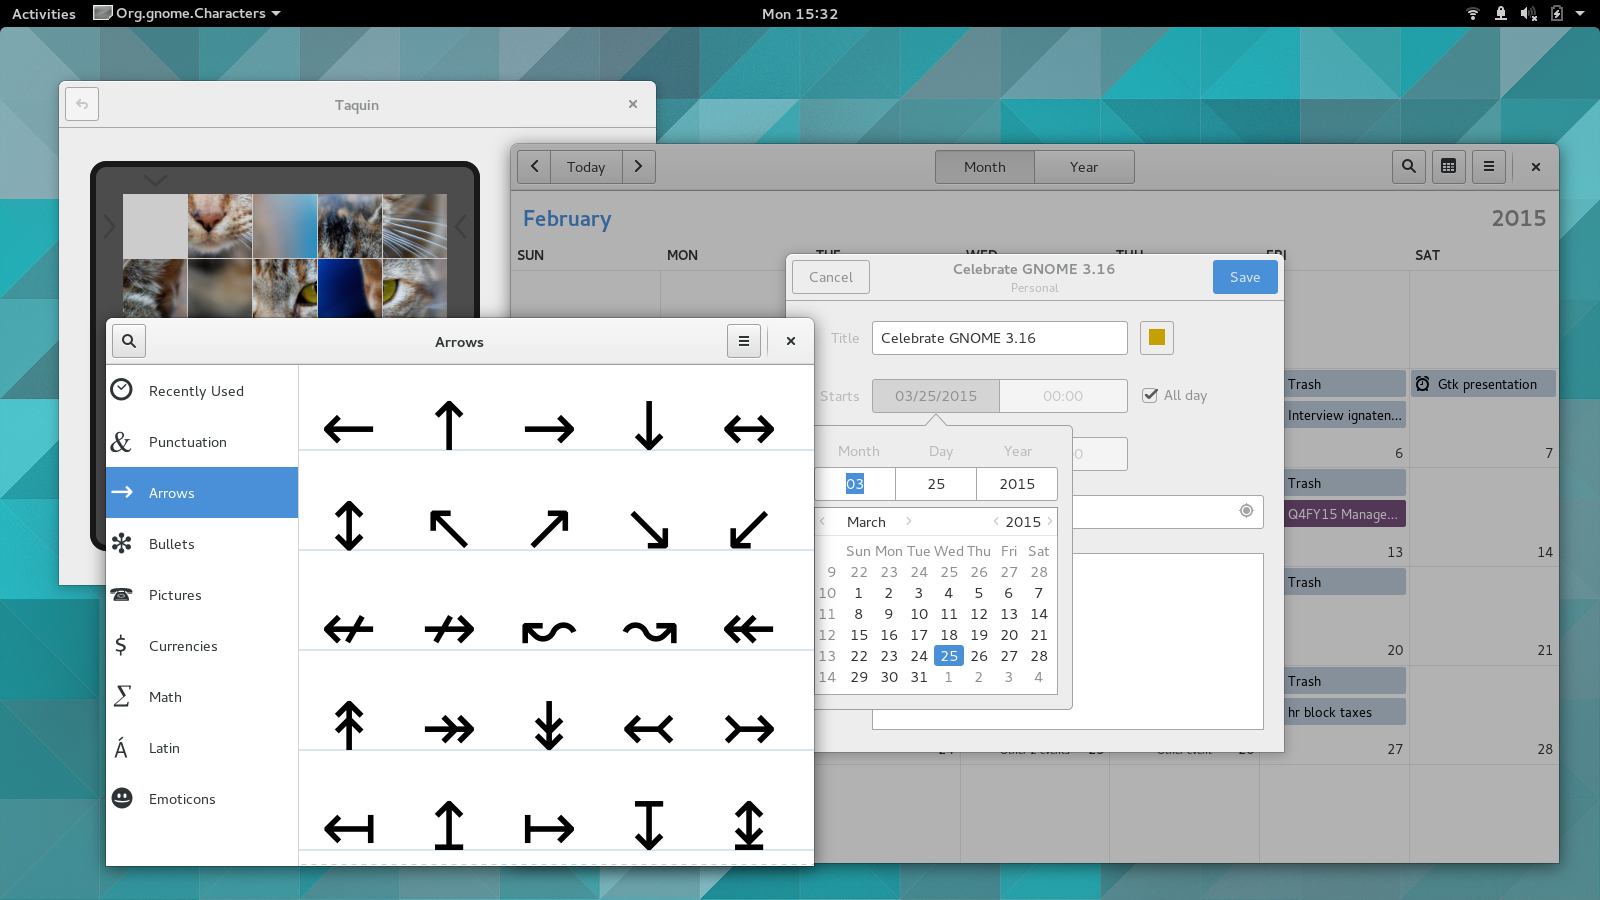
\includegraphics [width=\textwidth]{image/mclasen-new-apps.png}
    \fonte{Matias Clasen}
  \end{center}
\end{figure}

A plataforma GNOME e seus aplicativos centrais são baseados no toolkit GTK. O
GTK + é formado por um conjunto de ferramentas multi-plataforma para criar
interfaces gráficas de usuário. Por oferecer um conjunto completo de widgets é
adequado para projetos desde pequenas ferramentas pontuais até suítes completas
de aplicativos \cite{gtk-org}.

\section{Software livre e o desenvolvimento contínuo}

Uma das característica das plataformas de código aberto é a distribuição de
esforços em prol do constante desenvolvimento e melhoria. A pluralidade de
opiniões e idéias eleva o patamar das discussões e permite com que vários pontos
de vista sejam levados em consideração na evolução da plataforma.

Apesar dos prós existentes na distribuição de esforços também existem os contras
-- Projetos que são desenvolvidos paralelamente nem sempre avançam na mesma
velocidade. O contra fica mais sério quando um projeto depende do outro, como é
o caso de toolkits e programas que consomem suas APIs.

Quando ocorrem mudanças na interface de programação de uma framework ou
biblioteca, softwares dependentes tem de se adaptar as mudanças. O efeito
cascata provocado pela propagação de alterações na malha de softwares
dependentes não é incomum, e já foi objeto de estudo \cite{yau1978ripple}.

\section{Impactos na consistência e usabilidade}

Além dos aplicativos centrais, geralmente garantidos de acompanhar a evolução
da plataforma -- sua ergonomia e visual -- existe uma vasta gama de aplicações
tanto de código aberto quanto proprietárias disponíveis para atender as mais
variadas necessidades.

A grande maioria das aplicações GTK+ são mantidas pela comunidade de software
livre, e se não atualizadas podem ficar defasadas em usabilidade, ergonomia e
consistência com a plataforma. \citeonline{shneiderman1992designing} descreve
a usabilidade como uma combinação das seguintes características:

\begin{itemize}
    \item Facilidade de aprendizado
    \item Alta velocidade de operação
    \item Baixa taxa de erros
    \item Satisfação do usuário
    \item Retenção de usuários pelo tempo
\end{itemize}

Em prol da usabilidade a maioria dos toolkits aplica um modelo próprio de
apresentação, organização, interação e estilização de widgets, atendendo aos
requisitos do tipo de ambiente onde é executado (desktop, tablet e celular).

\section{HIG ou Human Interface Guidelines}

Divulgado no ano de 2014, acompanhando a versão 3.14 da plataforma GNOME, sob o
título de Human Interface Guidelines, o conjunto de padrões de design
oficialmente promovido pela GNOME Foundation busca promover a máxima integração
de interfaces gráficas GTK+ na plataforma GNOME.

\begin{citacao}
    Se você é um desenvolvedor com experiência limitada de design o HIG foi
    planejado para auxiliar você a criar facilmente uma interface de usuário
    efetiva. Para designers, o HIG provê uma introdução as possibilidades ao
    usar o GTK+, assim como padrões de design que são usados nos aplicativos
    GNOME \cite{gnome314hig}.
\end{citacao}

O HIG, como também é chamado, é uma literatura ilustrada de diretrizes
recomendadas no desenvolvimento de interfaces gráficas que utilizem o toolkit,
com o intuito de reforçar a consistência visual e integração com o ambiente
GNOME. A figura \ref{gnome-hig-patterns} ilustra alguns dos padrões de design
documentados pelo HIG.

\begin{figure}[htb]
  \begin{center}
    \caption{\textbf{Padrões e suas aplicações}}
    \label{gnome-hig-patterns}
    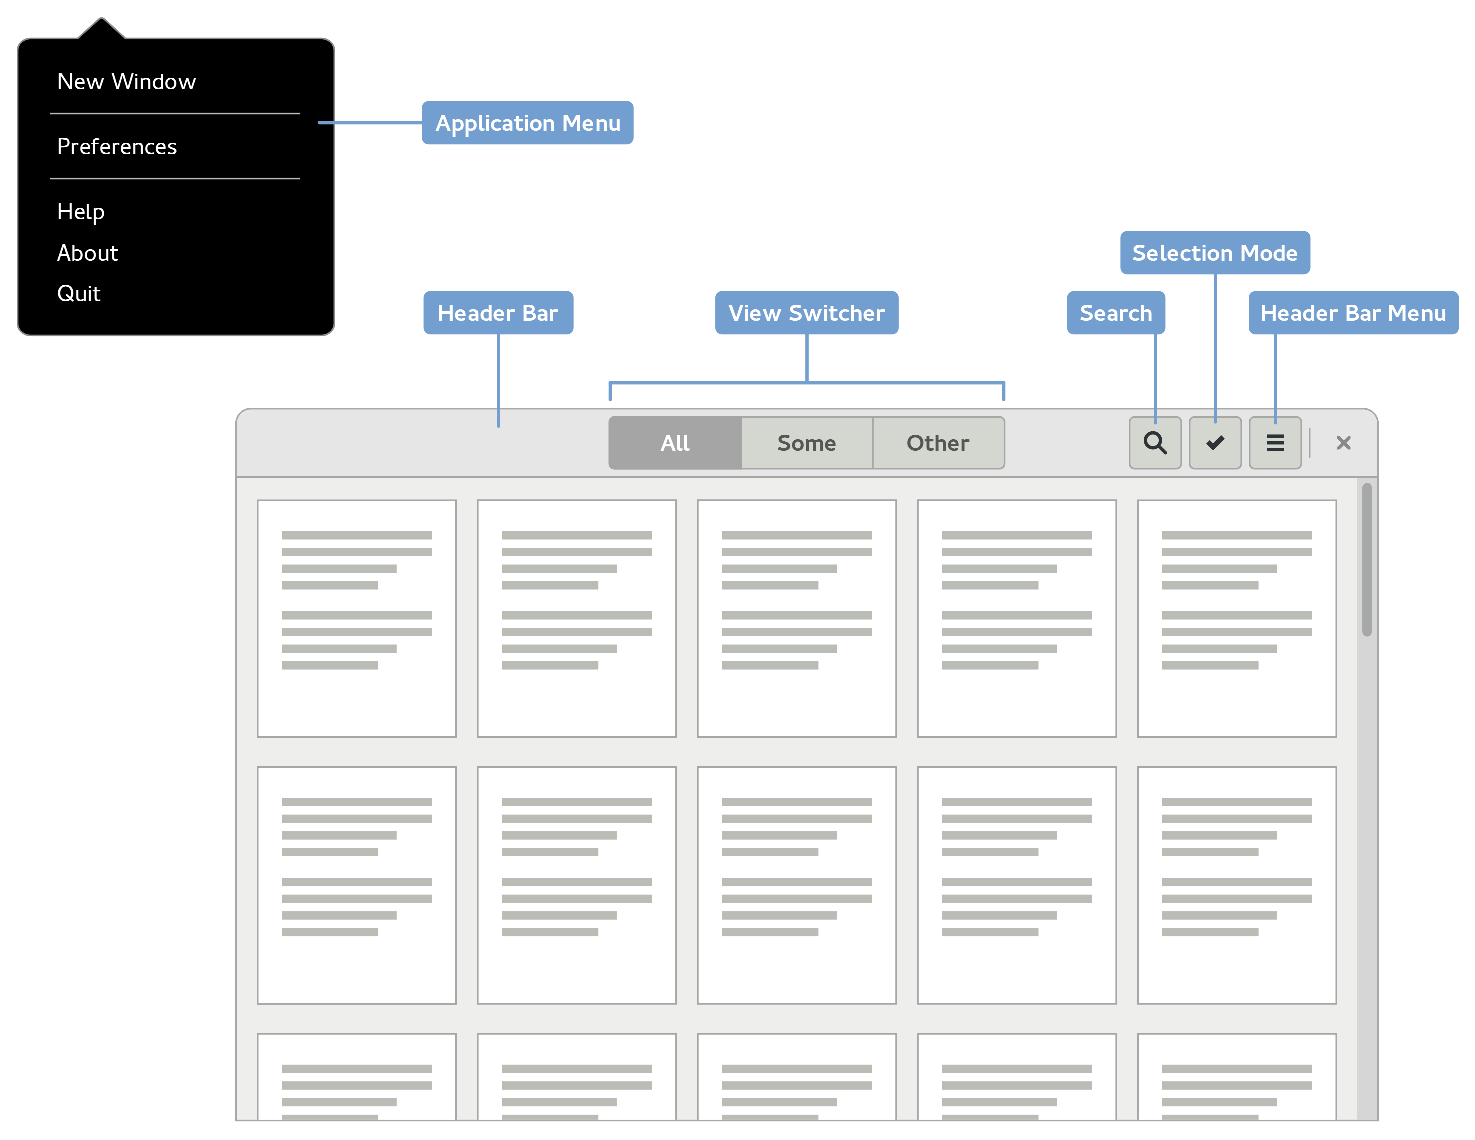
\includegraphics[width=\textwidth]{image/hig/patterns.eps}
    \fonte{GNOME 3.16 HIG - Patterns}
  \end{center}
\end{figure}

Dentre os objetivos do HIG estão a transmissão das metas de design de alto nível
e estratégicas da experiência GNOME e a comunicação das diretrizes de design
essenciais, de uma forma clara, e viva, acompanhando a evolução da plataforma
\citeonline{day2015wiki}.

\section{Estudo de caso: Transmission}

Um aplicativo famoso disponível para a plataforma GNOME é o cliente de
BitTorrent Transmission \cite{transmission282}. Aclamado pela sua simplicidade,
o aplicativo é utilizado para compartilhar arquivos através da internet.

Utilizando-se de uma configuração padrão funcional e poucos cliques para
configurar funcionalidades avançadas a utilização do cliente de torrent
Transmission foi projetada para ser fácil e poderosa
\cite{transmission-about}.

A primeira versão do Transmission foi lançada em Setembro de 2005, já com uma
interface gráfica baseada em GTK+, projetada sob as recomendação do HIG
da época, publicada digitalmente em formato de livro \cite{gnome221hig}.

\begin{figure}[htb]
  \begin{center}
    \caption{\textbf{Transmission 2.28 no GNOME 3.16}}
    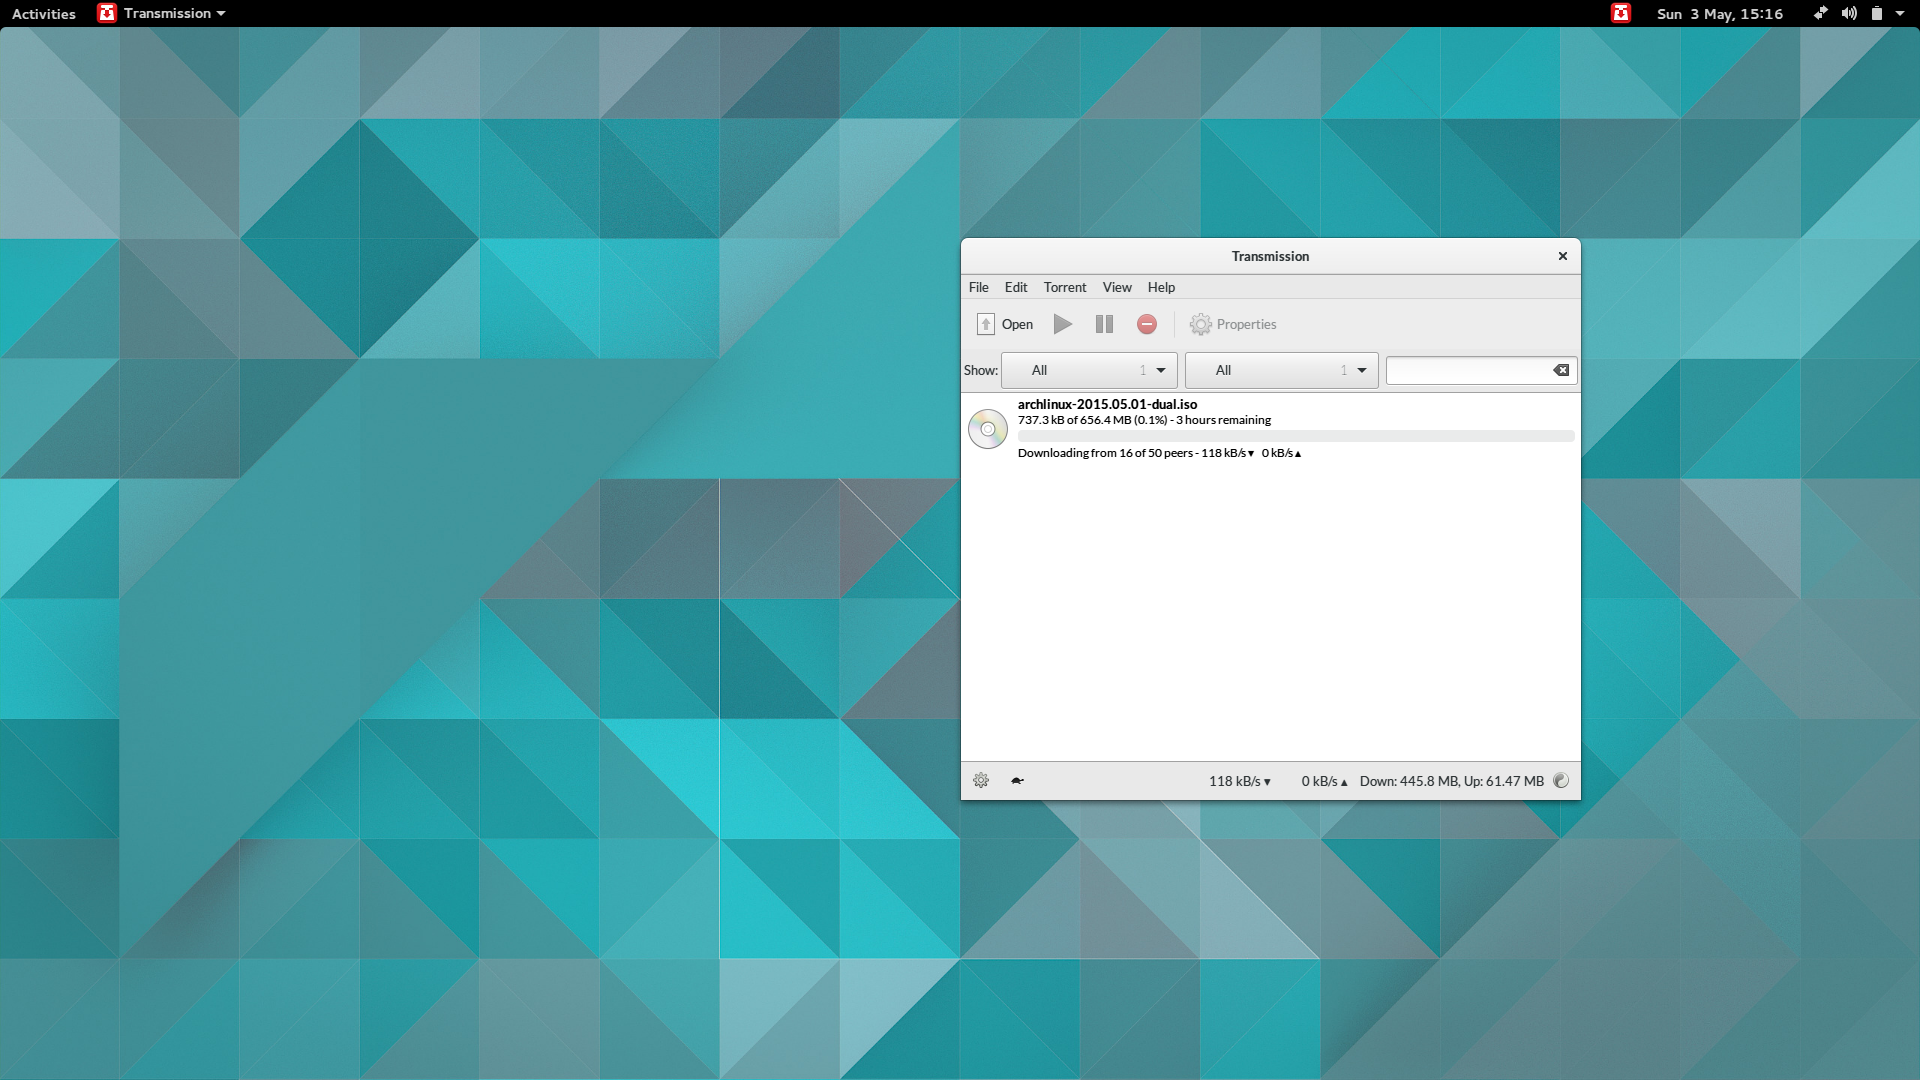
\includegraphics [width=\textwidth]{image/transmission/282-master/main-window.png}
    \label{transmission-master}
    \fonte{Do autor}
  \end{center}
\end{figure}


\chapter{PROCEDIMENTOS METODOLÓGICOS}

A presente pesquisa aplicada foi desenvolvida através da exploração de casos de
uso tanto da evolução de aplicativos centrais da plataforma GNOME quanto padrões
de design utilizados em outras versões do cliente de torrent Transmission.

Segundo \citeonline{jung2003metodologia}, o objetivo da pesquisa aplicada é
gerar inovação frente a uma demanda ou necessidade, e seu desenvolvimento
consiste na utilização dos conhecimentos adquiridos na pesquisa básica
associados a pesquisa tecnológica, com a finalidade de obter aplicações
práticas.

O produto final desta pesquisa se concretiza na forma de um protótipo funcional
de interface gráfica compatível com os padrões definidos no HIG 3.14 para o
cliente de torrent Transmission.

\section{Estudo longitudinal dos padrões de design nas aplicações}
\label{sec:chronologic-analysis}

Através de pesquisa exploratória com o objetivo de avaliar o processo de
evolução da plataforma GNOME e seu design, foram identificadas aplicações
centrais do GNOME 3.16 que já implementam os padrões de design definidos pelo
HIG \cite{gnome314hig}.

\citeonline{jung2003metodologia} caracteriza a pesquisa exploratória pela
extração de conhecimento sobre um dado fenômeno, sem grande teorização, visando
descobrir práticas e diretrizes alternativas ao conhecimento existente.

Foram escolhidas três aplicações centrais a serem analisadas. Pelo papel
significativo desempenhado na experiência GNOME foram selecionadas as seguintes
aplicações:

\begin{itemize}
    \item Nautilus -- Navegador de Arquivos
    \item Evince -- Visualizador de Documentos Digitais
    \item Gedit -- Editor de Arquivos de Texto
\end{itemize}

Com propósito de avaliar a dinâmica do processo de design do GNOME ao longo do
tempo, um estudo de caráter longitudinal foi elaborado nas três aplicações
escolhidas, através da comparação de duas versões distantes do GNOME e das
aplicações centrais escolhidas.

A montagem do ambiente necessário para a execução do estudo longitudinal foi
facilitada pela distribuição oficial de sistemas operacionais com todo software
necessário para uma experiência GNOME básica, prontos para usar através da
transferência para uma mídia inicializável \cite{gnome2015promo-usb}. Detalhadas
na \autoref{gnome-versions} estão as informações das versões escolhidas, dentre
as disponíveis para estudo.

A soma de verificação de cada arquivo foi utilizada para checar a integridade do
sistema operacional, e todas aplicações foram analisadas na versão oficial --
sem alterações na configuração do sistema, troca de temas, fontes, etc.

\begin{table}[htb]
\ibgetab{
  \caption{Sistemas operacionais e versões do GNOME}
  \label{gnome-versions}
}{
  \begin{tabularx}{\textwidth}{ | l | l | l | X | }
  \hline
  Versão do GNOME & Data de Modificação & Nome do arquivo & Soma de Verificação \\
  \hline
  3.6.0 & 08/10/2012 & GNOME-3.6.0.iso       & MD5:
                                               753c99ce2342f658
                                               65c1f74bc3722e44 \\
  \hline
  3.16  & 25/03/2015 & gnome-3.16.x86-64.iso & SHA256:
                                               4a6185a0aca89f15
                                               8f769d76d5a0086f
                                               0f1e9d709a5d80cd
                                               cf2b0d52d67ab2b2 \\
  \hline
  \end{tabularx}
}{
  \fonte{\cite{gnome2015promo-usb}}
}
\end{table}

Dentre os diversos padrões de design especificados pelo HIG
\cite{hig314patterns} foram selecionados cinco padrões de interesse a serem
analisados no estudo:

\begin{enumerate}
  \item Menu da Aplicação
  \item Janela Primária
  \item Barra de Título
  \item Comutador de Visão
  \item Busca
\end{enumerate}

As variáveis observadas no estudo incluiram, porém não se limitaram a (i) área
útil vs controles, onde foi analisada a razão entre a quantidade de pixels de
área útil versus controles da aplicação e (ii) relocação de funcionalidade,
onde foram analisadas mudanças operacionais em um mais elementos de interface,
sendo estas de caráter quantitativo e qualitativo, respectivamente.

A obtenção da razão área útil versus controles foi feita através da medição em
pixels da janela principal de cada aplicativo Foi considerada área útil a área
do aplicativo na qual a informação principal é apresentada, conforme
exemplificado na \autoref{workarea-chrome-ratio}. No caso do Nautilus, a lista
de arquivos é a área principal, do Evince, o documento apresentado, e no caso do
Gedit, a área de edição de texto.

\begin{figure}[h!]
  \begin{center}
    \caption{\textbf{Medição da razão área útil vs controles}}
    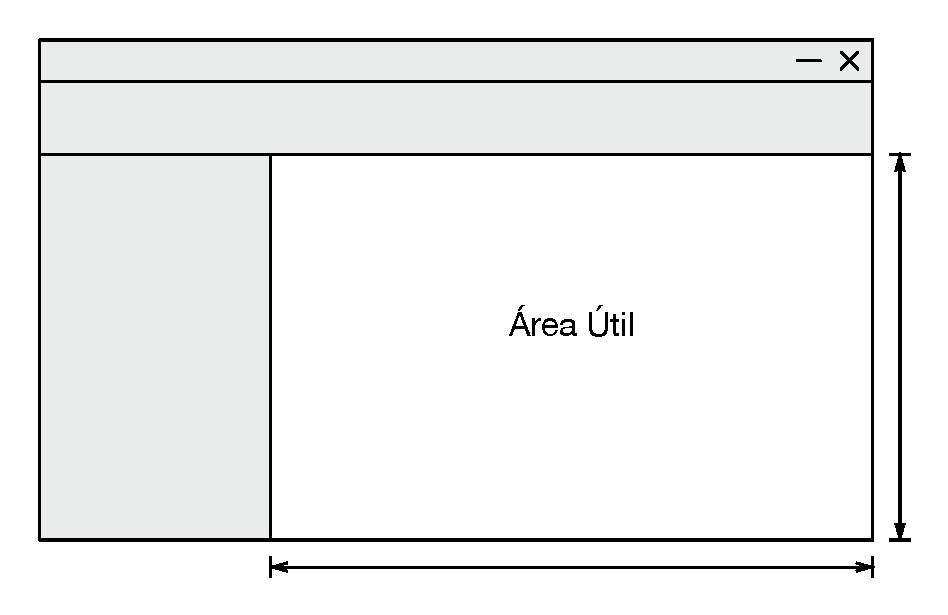
\includegraphics[scale=0.7]{image/workarea-chrome-ratio.eps}
    \fonte{Do Autor}
    \label{workarea-chrome-ratio}
  \end{center}
\end{figure}

A relocação de funcionalidades analisou a transição de um elemento de interface,
onde um menu, por exemplo, pode ter sido transformado em um botão, movido para
outro local, etc.

\section{Proposição de melhorias na interface do Transmission}

\citeonline{de2009client} afirmam que a prototipação de interfaces é uma técnica
de evolução de design que tem como base a constante interação e avaliação dos
resultados. \citeonline[p. 2]{baumer1996user} classifica e separa em quatro
classes os protótipos de interfaces gráficas:

\begin{enumerate}
  \item De apresentação
  \item Funcional
  \item Experimental
  \item Piloto
\end{enumerate}

Pela (i) maleabilidade de implementar estrategicamente ambas interface gráfica e
funcionalidade de um programa, com o propósito de averiguar o funcionamento de
um conceito e (ii) pelo fato do Transmission permitir alterações em seu código-
fonte através de sua licença GPL o protótipo funcional foi escolhido como método
experimental para a geração de propostas de melhorias na interface do
Transmission.

O protótipo funcional foi gerado através de alterações experimentais no código-
fonte do Transmission objetivando modificar sua interface gráfica utilizando
como base as tendências encontradas no estudo logitudinal das aplicações
centrais e também as diretivas estabelecidas no HIG.


\chapter{RESULTADOS E DISCUSSÕES}

O cenário ilustrado na \ref{transmission-at-gnome} evidencia que a adaptação
proposta na interface do Transmission provê maior harmonia com outros
aplicativos da plataforma GNOME.

\begin{figure}[htb]
  \begin{center}
    \caption{\textbf{Transmission no GNOME 3.16}}\label{transmission-at-gnome}
    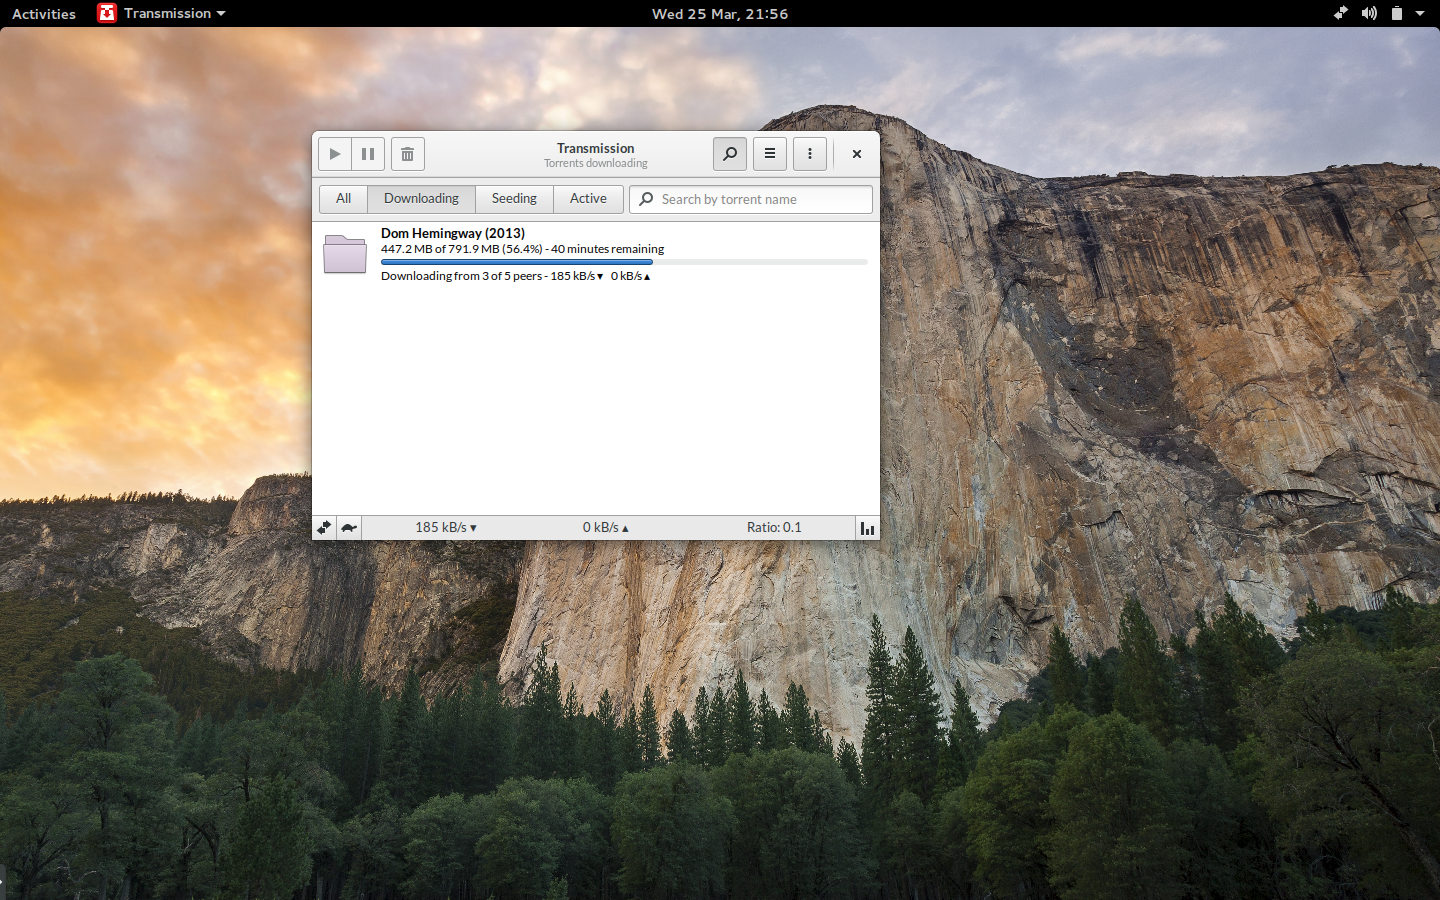
\includegraphics [scale=0.2]{image/transmission-gtk3-main.png}
    \label{transmission-at-gnome}
  \end{center}
\end{figure}

\section{A evolução das aplicações centrais analisadas}

A análise das aplicações centrais do GNOME trouxe resultados efetivos sobre a
transição gráfica e funcional dos principais widgets utilizados pela aplicação.

Um ítem notável foi a redução na utilização de espaço vertical em aplicações
centrais. \citeonline{day2014saving} analisa a redução do uso vertical de espaço
em várias versões do Nautilus e apresenta a seguinte tabela:

\begin{center}
    \begin{tabular}{ | l | l | } 
    \hline
    Versão do Nautilus & Moldura Vertical \\ \hline
    2.22 & 171 pixels \\
    3.0  & 116 pixels \\
    3.6  & 70 pixels \\
    3.12 & 48 pixels \\
    \hline
    \end{tabular}
\end{center}

Observou-se que o fenômeno se repete em todas as aplicações centrais analisadas:

% \begin{figure}[htb]
%   \begin{center}
%     \caption{\textbf{Barra de Cabeçalho - Nautilus}}
%     \includegraphics[width=\textwidth]{image/benchmark/nautilus-headerbar.png}
%     \label{nautilus-headerbar}
%   \end{center}
% \end{figure}

% \begin{figure}[htb]
%   \begin{center}
%     \caption{\textbf{Barra de Cabeçalho - Evince}}
%     \includegraphics[width=\textwidth]{image/benchmark/evince-headerbar.png}
%     \label{evince-headerbar}
%   \end{center}
% \end{figure}

% \begin{figure}[htb]
%   \begin{center}
%     \caption{\textbf{Barra de Cabeçalho - Gedit}}
%     \includegraphics[width=\textwidth]{image/benchmark/gedit-headerbar.png}
%     \label{evince-headerbar}
%   \end{center}
% \end{figure}

\section{Barra de Título}

Um dos elementos de interface mais notáveis é a barra de título. Até então
desenvolvedores tinham pouco ou nenhum controle sobre elas por questões de
compatibilidade de software. Com o surgimento do conceito de `Header Bars', 
as barras de título ganharam  botões, caixas de texto, sliders, etc.

\section{Barra de Filtros}

Mostrar todos os controles de uma só vez torna a aplicação mais díficil de usar.
Portanto é necessário 

\section{Limites Globais de Upload/Download}

\section{Botão Limite de velocidade}

\section{Estísticas da barra de status}


\chapter{CONCLUSÃO}

Os resultados obtidos através desta pesquisa foram de grande satisfatoriedade,
tanto em relação ao seu processo de desenvolvimento, qual trouxe conhecimentos
valiosos, cumprindo com todos seus objetivos, quanto em relação ao resultado em
sí, qual trouxe maior harmonia para a utilização do Transmission na plataforma
GNOME.

Em relação a sua titulação, o autor acredita que o embasamento nas aplicações
centrais que já implementam os padrões definidos pelo HIG fez com que o redesign
esteja de acordo com este guia.

Como perspectiva de trabalhos futuros, o presente autor espera que a motivação
desta pesquisa seja inspiração para o redesign de outras aplicações que
necessitem da mesma atenção, na expectativa de que este trabalho contribua
positivamente para o desenvolvimento de trabalhos futuros.


\bibliography{content/referencias}

\label{nropaginas}

\printindex

\end{document}
